\documentclass{article}
\usepackage{tikz}
\usetikzlibrary{shapes.geometric, arrows, positioning, calc}

\begin{document}
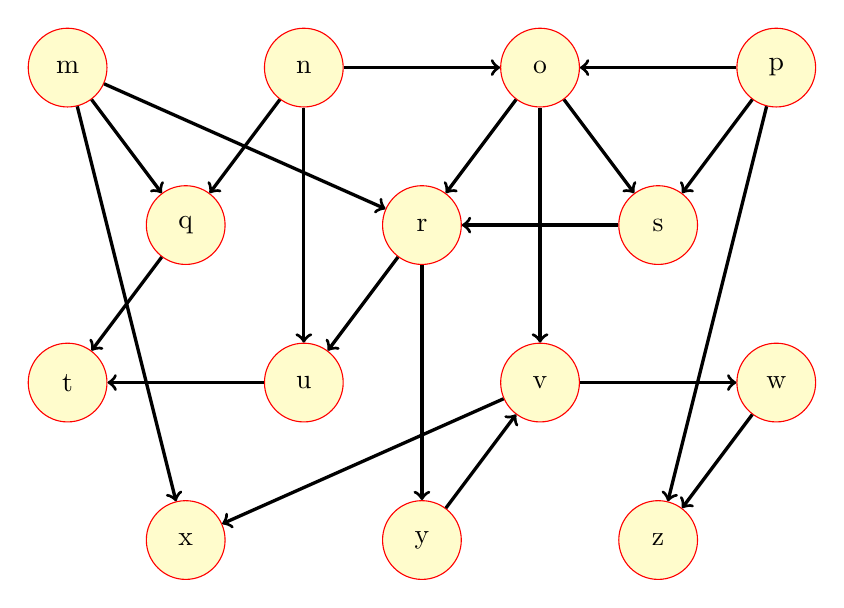
\begin{tikzpicture}
\node[circle, draw=red, fill=yellow!20,minimum size=1cm] 
(t) at (0, 0) {t};
\node[circle, draw=red, fill=yellow!20,minimum size=1cm] (u) at (3, 0) {u};
\node[circle, draw=red, fill=yellow!20,minimum size=1cm] (v) at (6, 0) {v};
\node[circle, draw=red, fill=yellow!20,minimum size=1cm] (w) at (9, 0) {w};
\node[circle, draw=red, fill=yellow!20,minimum size=1cm] (x) at (1.5, -2) {x};
\node[circle, draw=red, fill=yellow!20,minimum size=1cm] (y) at (4.5, -2) {y};
\node[circle, draw=red, fill=yellow!20,minimum size=1cm] (z) at (7.5, -2) {z};
\node[circle, draw=red, fill=yellow!20,minimum size=1cm] (q) at (1.5, 2) {q};
\node[circle, draw=red, fill=yellow!20,minimum size=1cm] (r) at (4.5, 2) {r};
\node[circle, draw=red, fill=yellow!20,minimum size=1cm] (s) at (7.5, 2) {s};
\node[circle, draw=red, fill=yellow!20,minimum size=1cm] (m) at (0, 4) {m};
\node[circle, draw=red, fill=yellow!20,minimum size=1cm] (n) at (3, 4) {n};
\node[circle, draw=red, fill=yellow!20,minimum size=1cm] (o) at (6, 4) {o};
\node[circle, draw=red, fill=yellow!20,minimum size=1cm] (p) at (9, 4) {p};

%connections
\draw[->,very thick] (m) to (q);
\draw[->,very thick] (m) to (r);
\draw[->,very thick] (m) to (x);
\draw[->,very thick] (n) to (q);
\draw[->,very thick] (n) to (u);
\draw[->,very thick] (n) to (o);
\draw[->,very thick] (o) to (r);
\draw[->,very thick] (o) to (v);
\draw[->,very thick] (o) to (s);
\draw[->,very thick] (p) to (s);
\draw[->,very thick] (p) to (z);
\draw[->,very thick] (p) to (o);
\draw[->,very thick] (q) to (t);
\draw[->,very thick] (r) to (u);
\draw[->,very thick] (r) to (y);
\draw[->,very thick] (s) to (r);
\draw[->,very thick] (u) to (t);
\draw[->,very thick] (v) to (x);
\draw[->,very thick] (v) to (w);
\draw[->,very thick] (y) to (v);
\draw[->,very thick] (w) to (z);
\end{tikzpicture}
\end{document}